% 8185: Quant Ellen PS3

\documentclass[12pt]{article}
%\usepackage[T1]{fontenc}
%\usepackage{lipsum}
\renewcommand{\baselinestretch}{1.2} 
\usepackage{graphicx}
\usepackage{hyperref}
\hypersetup{
    colorlinks=true,
    urlcolor=blue,
    citecolor=blue
}
\usepackage[export]{adjustbox}
\usepackage{subcaption}
\usepackage{amsmath}
\usepackage{amsfonts}
\usepackage{geometry}
\setcounter{MaxMatrixCols}{20}
\geometry{a4paper,
 left=3cm,right=3cm,
 top=1.5cm, bottom=1.5cm}

\usepackage{natbib}
\bibliographystyle{apalike}

%\usepackage{natbib}
%setcitestyle{authoryear,open={(},close={)}}
\graphicspath{ {../figs/} }

\begin{document}
%\thispagestyle{myheadings}
%\markright{Indian Statistical Institute, New Delhi\hfill }

\title{Econ 8185: Quant PS3}
\author{Bipul Verma}
\date{\today}
\maketitle

%\tableofcontents{}
\abstract{The present document uses Kalman Filter to estimate the coefficients and shock variance.}

\vspace{8cm}

%\begin{center}
%\includegraphics[scale=0.4]{isi_logo.png}
%\end{center}
%\begin{center}
%\begin{Large}
%INDIAN STATISTICAL INSTITUTE, NEW-DELHI.
%\end{Large}
%\end{center}


\newpage

\section{State Space Models and Kalman Filter}
The linear state space model assumes that observed time series $\{y_t\}$ is a linear function of state variable $\alpha_t$ (usually unobserved). It is further assumed that the state variable $\alpha_t$ follows a first order vector autoregressive process. Mathematically the \textit{state space} system is:
\begin{align}
y_t = Z\alpha_t + \epsilon_t \\
\alpha_t = T \alpha_{t-1} + \eta_t
\end{align}
where $\epsilon_t$, $\eta_t$ are assumed to be mean $0$ white noise. Specifically,
\begin{gather*}
\mathbb{E}[\epsilon_t] =0, \mathbb{E}[\eta_t] =0, \mathbb{E}[\epsilon_t \eta_s]=0\\
\mathbb{E}[\epsilon_t \epsilon_t'] = H \\
\mathbb{E}[\eta_t \eta_t'] = Q.
\end{gather*}
Equation $(1)$ is also called as the \textit{Measurement or Observer equation}, while equation $(2)$ as the \textit{transition equation.} It turns out that a lot of models can be put in state space representation. Once we have the state space representation, the Kalman Filter is a system of two equations- the \textit{predicting equation} and the \textit{updating equation}. Mathematically, the Kalman Filter consists of:
\begin{align}
\hat{\alpha}_{t|t-1} = T \hat{\alpha}_{t-1}\\
\hat{\alpha}_{t+1|t} = T \hat{\alpha}_{t|t-1} + K_t i_t \\
y_t = \underbrace{Z \hat{\alpha}_{t|t-1}}_{\hat{y}_{t|t-1}} + i_t
\end{align}
where $\hat{\alpha}_{t|t-1}$ is an estimate of unobserved state vector. The matrix $K_t$ is \textit{Kalman gain}, $i_t = y_t - \hat{y}_{t|t-1} = y_t - Z \hat{\alpha}_{t|t-1} $ is an \textit{innovation} which is the difference between the observable and its prediction. The idea being that the actual observed $y_t$ consists of a component that we were able to predict $\hat{y}_{t|t-1}$ and \textit{innovation} $i_t$. It is to note that the prediction of $y_t$ i.e $\hat{y}_{t|t-1}$ is entirely based on the prediction of state $\hat{\alpha}_{t|t-1}$ (since $\hat{y}_{t|t-1} = Z \hat{\alpha}_{t|t-1}$). Kalman filter thus evolves around predicting $(\hat{\alpha}_{t|t-1})$  and updating the prediction of the state vector$(\hat{\alpha}_{t+1|t}).$ At time $t$ before we have actually observed $y_t$, our information set consists of lagged values of $y: (y_0, y_1, \dots, y_{t-1}).$ Based on this information, we begin by making the best guess for the underlying state. From the law of motion of state we have:
\begin{align*}
\hat{\alpha}_{t|t-1} = \mathbb{E}[\alpha_t | (y_0, y_1, \dots, y_{t-1}) ] = T\mathbb{E}[\alpha_{t-1}|(y_0, y_1, \dots, y_{t-1})] + \underbrace{\mathbb{E}[\eta_t|(y_0, y_1, \dots, y_{t-1})]}_{0}.
\end{align*}

Define:
\begin{align*}
\hat{\alpha}_{t-1} = \mathbb{E}[\alpha_{t-1}| y_0, y_1, \dots , y_{t-1}].
\end{align*}

Combining the above two equation gives us back equation $(3)$, which is our prediction  for the state vector, which then gives the prediction for observable $\hat{y}_{t|t-1}$. Now we want to update our prediction in after we have actually observed $y_t$. But before that we'll define some objects which will be used in our updation equation.

At time $t$, we can write the variance of prediction error as:
\begin{align*}
P_{t-1} = \mathbb{E}[(\alpha_{t-1} - \hat{\alpha}_{t-1})(\alpha_{t-1} - \hat{\alpha}_{t-1})'].
\end{align*}
We see that our estimate $\hat{\alpha}_{t|t-1} = T \hat{\alpha}_{t-1}$ is a function of lagged values of $y$. The conditional variance of prediction error is given by:
\begin{align*}
P_{t|t-1} &  = \mathbb{E}[(\alpha_t - \hat{\alpha}_{t|t-1})(\alpha_t - \hat{\alpha}_{t|t-1})']\\
& = \mathbb{E}[(T\alpha_{t-1} + \eta_t - T\hat{\alpha}_{t-1})(T\alpha_{t-1} + \eta_t - T\hat{\alpha}_{t-1})']\\
& = \mathbb{E}[(T(\alpha_{t-1}-\hat{\alpha}_{t-1})+ \eta_t)(T(\alpha_{t-1}-\hat{\alpha}_{t-1})+ \eta_t)'] \\
& = T\mathbb{E}[(\alpha_{t-1}-\hat{\alpha}_{t-1})(\alpha_{t-1}-\hat{\alpha}_{t-1})']T'+ \mathbb{E}[\eta_t\eta_t']\\
& = TP_{t-1}T' + Q.
\end{align*}
Here we have made use of the fact that $(\alpha_{t-1}-\hat{\alpha}_{t-1})$ and $\eta_t$ are uncorrelated. In a similar spirit we can calculate the variance of innovation $i_t = y_t - \hat{y_{t|t-1}} = y_t - Z \hat{\alpha}_{t|t-1}].$ The conditional variance of innovation is: 
\begin{align*}
F_t & = \mathbb{E}[i_t i_t'] \\
 & = \mathbb{E}[(y_t - Z \hat{\alpha}_{t|t-1})(y_t - Z \hat{\alpha}_{t|t-1})']\\
& = \mathbb{E}[(Z \alpha_t - Z \hat{\alpha}_{t|t-1})( Z \alpha_t - Z \hat{\alpha}_{t|t-1})']\\
& = Z P_{t|t-1}Z' + H.
\end{align*}
Similarly, the covariance of $i_t$ with prediction (state) error is:
\begin{align*}
G_t & = \mathbb{E}[(y_t - \hat{y}_{t|t-1})(\alpha_t - \hat{\alpha}_{t|t-1})']\\
& = \mathbb{E}[(Z\alpha_t - Z\hat{\alpha}_{t|t-1} + \epsilon_t)(\alpha_t - \hat{\alpha}_{t|t-1})'] \\
& = ZP_{t|t-1}.
\end{align*}
Note that before we actually observe $y_t$, conditional on the information set $(y_0, y_1, \dots, y_{t-1})$, all the matrices $P_{t-1}, P_{t|t-1}, F_t, G_t$, are known.

For jointly Normal random variable $X$ and $Y$ with the var-covariance matrix given by:
\begin{align*}
\Sigma = \begin{bmatrix}
\Sigma_{XX} & \Sigma_{XY} \\
\Sigma_{XY} & \Sigma_{YY}
\end{bmatrix},
\end{align*}
the conditional expectation of $Y$ given $X$ is given by:
\begin{align*}
\mathbb{E}[Y|X] = \mathbb{E}[Y] + \Sigma_{XY} \Sigma_{XX}^{-1}(X - \mathbb{E}[X]),
\end{align*}
and the conditional variance is given by:
\begin{align*}
Var[Y|X] = \mathbb{E}[(Y - E[Y|X])^2] = \Sigma_{YY} - \Sigma_{YX}\Sigma_{XX}^{-1}\Sigma_{XY}.
\end{align*}
It then follows from the above formula that:
\begin{multline*}
\mathbb{E}[\alpha_t| (y_0, y_1, \dots, y_{t-1}), y_t] = \mathbb{E}[\alpha_t|(y_0, y_1, \dots, y_{t-1})] \\
+ Cov(\alpha_t, y_t)Var(y_t)^{-1}(y_t - \mathbb{E}[y_t | (y_0, y_1, \dots, y_{t-1})]).
\end{multline*}
\begin{align*}
Cov(\alpha_t, y_t ) &  = \mathbb{E}[(\alpha_t - E[\alpha_t|(y_0, y_1, \dots, y_{t-1})])(y_t - E[y_t | (y_0, y_1, \dots, y_{t-1})])']\\
& = \mathbb{E}[(\alpha_t - \hat{\alpha}_{t|t-1})(y_t - \hat{y}_{t|t-1})']\\
& = P_{t|t-1}Z' \\
Var(y_t) & = \mathbb{E}[(y_t - E[y_t|(y_0, y_1, \dots, y_{t-1})])(y_t - E[y_t|(y_0, y_1, \dots, y_{t-1})']\\
& = \mathbb{E}[(y_t - \hat{y}_{t|t-1})(y_t - \hat{y}_{t|t-1} )']\\
& = ZP_{t|t-1}Z' + H.
\end{align*}
Thus the updation equation is given by:
\begin{align*}
\hat{\alpha}_t & = \hat{\alpha}_{t|t-1} + P_{t|t-1}Z'(ZP_{t|t-1}Z' + H)^{-1}(y_t - \hat{y}_{t|t-1})\\
& =  \hat{\alpha}_{t|t-1} + G_t' (F_t)^{-1}(y_t - \hat{y}_{t|t-1}).
\end{align*}
Multiplying both sides of previous equation by T we get:
\begin{align*}
\hat{\alpha}_{t+1|t} = T\hat{\alpha}_{t|t-1} + K i_t
\end{align*}
where $K = TP_{t|t-1}Z'(ZP_{t|t-1}Z' + H)^{-1} = T G_t' (F_t)^{-1}$, and $i_t = y_t - \hat{y}_{t|t-1}$.
In a similar fashion using the conditional variance formula we get:
\begin{align*}
P_t = P_{t|t-1} - G_t'F_t^{-1}G_t.
\end{align*}

\subsection{Kalman Filter Implementation}
\begin{enumerate}
\item Begin with a guess for $\alpha_0$, $P_0$.  One can set $\alpha_0$ to be the unconditional mean of state vector, $P_0$ with the stationary $P$ that solves $P = TPT' + Q$. Set $\hat{\alpha}_{1|0} = T \alpha_0, P_{1|0} = TP_{0}T' + Q$.
\item Get:
\begin{enumerate}
\item $\hat{y}_{1|0} = Z\hat{\alpha}_{1|0}$
\item $i_1 = y_1 - \hat{y}_{1|0} $
\item $F_1 = ZP_{1|0}Z' + H, G_1 = ZP_{1|0}, K_1 = TG_1'F_1^{-1}$
\item $\hat{\alpha}_{2|1} = T \hat{\alpha}_{1|0} + K_1 i_1$
\item $P_{2|1} = T(P_{1|0} - G_1'F_1^{-1}G_1)T' + Q$
\item Go back to step $(a)$ increasing the time order by $1$ unit.
\end{enumerate}
\item Continue the recursion in this fashion to get sequence of $\{ \hat{\alpha}_{t|t-1} \}$, $\{i_t\}$ and $\{\hat{y}_{t|t-1}\}.$
\end{enumerate}

\subsection{Parametric Estimation using Log Likelihood}
To estimate the parameters we set the likelihood as:
\begin{align*}
\ln L = \sum_t \{ -\frac{n}{2} \ln 2\pi -\frac{1}{2}\ln |det(F_t)| - \frac{1}{2}i_t'F_t^{-1}i_t 
\end{align*}

\subsection{Application: HW3}
We'll write the processes in state space representation first.
\begin{enumerate}
\item $AR(1): x_t = \rho x_{t-1} + \epsilon_t$ \\

State: \hspace{4mm} $x_t = [\rho]x_{t-1} + \epsilon_t$ \\
Observation: $ x_t = [1]x_t$

\item $AR(2): x_t = \rho_1 x_{t-1} + \rho_2 x_{t-2} + \epsilon_t$\\

State: \hspace{4mm} $\begin{bmatrix} x_t \\ x_{t-1} \end{bmatrix} 
= \begin{bmatrix} 
\rho_1 & \rho_2 \\ 
1 & 0
\end{bmatrix}
\begin{bmatrix}
x_{t-1} \\ x_{t-2}
\end{bmatrix} + \begin{bmatrix}
1 \\ 0
\end{bmatrix} \epsilon_t $ \\
Observation: $ x_t = \begin{bmatrix} 1 & 0\end{bmatrix} \begin{bmatrix}x_t \\ x_{t-1}\end{bmatrix}$

\item $MA(1): x_t = \epsilon_t + \rho \epsilon_{t-1}$\\

State: \hspace{4mm} $\begin{bmatrix} \epsilon_t \\ \epsilon_{t-1} \end{bmatrix} 
= \begin{bmatrix} 
0 & 0 \\ 
1 & 0
\end{bmatrix}
\begin{bmatrix}
\epsilon_{t-1} \\ \epsilon_{t-2}
\end{bmatrix} + \begin{bmatrix}
1 \\ 0
\end{bmatrix} \epsilon_t $ \\
Observation: $ x_t = \begin{bmatrix} 1 & \rho \end{bmatrix} \begin{bmatrix}\epsilon_t \\ \epsilon_{t-1}\end{bmatrix}$

\item $Random Walk:$

State: \hspace{4mm} $\mu_t = [1]\mu_{t-1} + \eta_t$ \\
Observation: $x_t = [1]\mu_t + \epsilon_t.$

\end{enumerate}

\newpage
\subsection{Results}

\subsubsection{AR(1)}
We set $\rho = 0.6$ and $\sigma = 0.5$. We then simulate values of the $AR(1)$ process for 100 periods. 

\begin{figure}[h]
\centering
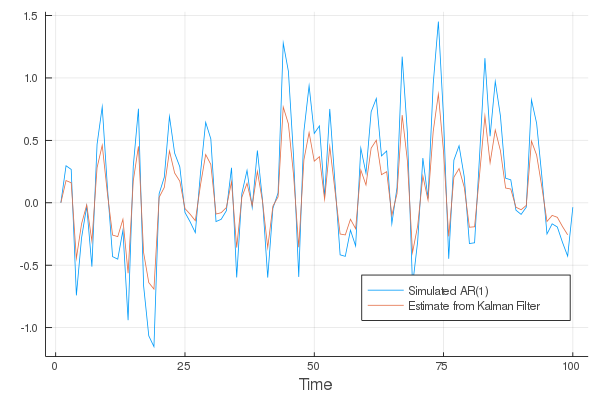
\includegraphics[scale=0.4]{AR1.png}
\caption{Simulated vs Filtered AR(1)}
\end{figure}

We note that given the required input matrices Kalman Filter closely follows the actual simulated $AR(1)$ process. We then use the log likelihood formula as given in section $1.2$ to calculate the likelihood of observing the simulated $AR(1)$ process. We then maximize the likelihood with respect to the $AR(1)$ parameters to get estimates for the parameters. The estimated parameters are:
$\hat{\rho} = 0.44, \hat{\sigma} = 0.48$ with 100 observation and $\hat{\rho} = 0.59, \hat{\sigma} = 0.48$ with 1000 observations. We note that the estimates are very close to original with 1000 data points. 

\subsubsection{AR(2)}
We set $\rho_1 = 0.3, \rho_2 = 0.4,$ and $\sigma=0.5$. We then simulate values for the $AR(2)$ process for 100 periods.
\begin{figure}[h]
\centering
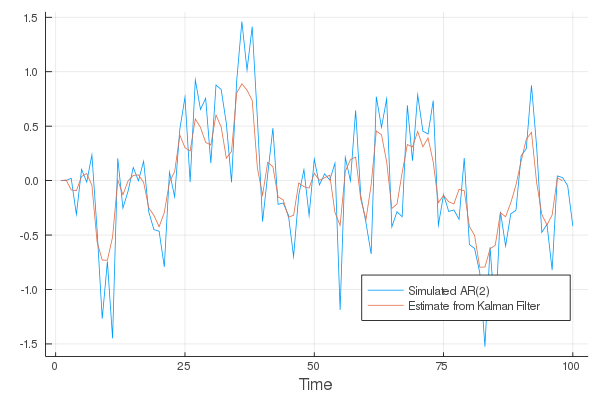
\includegraphics[scale=0.4]{AR2.png}
\caption{Simulated vs Filtered AR(2)}
\end{figure}

We note that the filtered process matches the simulated process well, except for instances where there are large spikes in the simulated process. The estimates from MLE estimates are: $\hat{\rho_1} = 0.43, \hat{\rho_2} = 0.34, \hat{\sigma} =0.49$ with 100 observation and $\hat{\rho_1} = 0.399, \hat{\rho_2} = 0.499, \hat{\sigma} =0.507$ with 1000 observations. We note that the estimates are very close to original with 1000 data points. 

\subsubsection{MA(1)}
We set the parameters $\rho = 0.7, \sigma= 0.8$ for $MA(1)$ process. We simulate the values for $MA(1)$ process for 100 periods.
\begin{figure}[h]
\centering
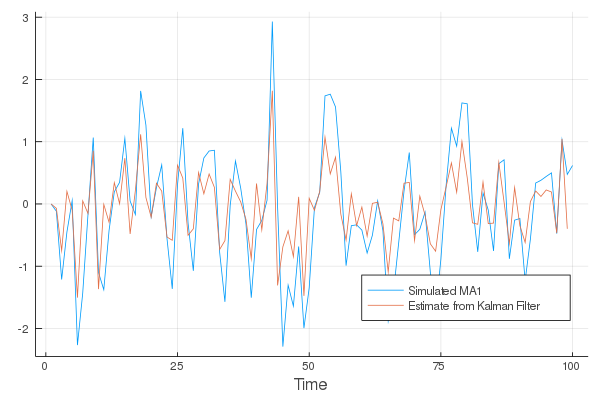
\includegraphics[scale=0.4]{MA1.png}
\caption{Simulated vs Filtered MA(1)}
\end{figure}

We note that the filtered process matches the simulated process well, except for instances where there are large spikes in the simulated process. The estimates from MLE estimates are: $\hat{\rho} = 0.79, \hat{\sigma} =0.83$ with 100 data points, and $\hat{\rho} = 0.694, \hat{\sigma} =0.812$ with 5000 observations . We note that the MLE estimates are close to the actual parameter values used for simulation with 5000 observations.

\subsubsection{Random Walk}
We set the parameters $\sigma_{\epsilon} = 0.8, \sigma_{\eta}= 0.6$ for Random Walk process. We simulate the values for Random Walk for 100 periods.
\begin{figure}[h]
\centering
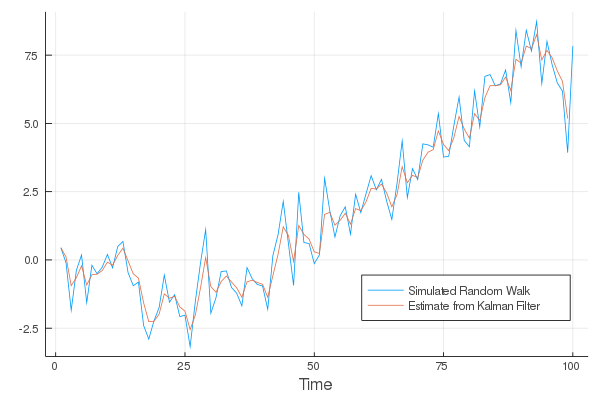
\includegraphics[scale=0.4]{RW.png}
\caption{Simulated vs Filtered Random Walk}
\end{figure}

We note that the filtered process matches the simulated process well, except for instances where there are large spikes in the simulated process. The estimates from MLE estimates are: $\hat{\sigma}_{\epsilon} = 0.85, \hat{\sigma}_{\eta}= 0.41$ with 100 observation, and $\hat{\sigma}_{\epsilon} = 0.81, \hat{\sigma}_{\eta}= 0.58$ with 5000 observations.  We note that the MLE estimates are close to the actual parameter values with 5000 observations.
%\newpage
%\bibliography{ref}

\end{document}